
\documentclass[aspectratio=169]{beamer}
\usetheme{metropolis}           % Use metropolis theme
\usepackage[utf8]{inputenc}
\usepackage{graphicx}
\usepackage{eso-pic}
\usepackage{graphics}
\usepackage{tikz}
\usepackage[export]{adjustbox}
\usepackage{multicol}
\usepackage{listings}
\usepackage{helvet}
\usepackage{booktabs}
\usepackage{threeparttable}
\usepackage{fontspec}
\usepackage{hyperref}
\hypersetup{urlcolor=DarkBlue}

\title{Topic 4 - Track 1 \newline Real Time Data Quality Checks}
\date{\today}
\author{Author of Session here!} % Name of author(s) of session here
\institute{Development Impact Evaluation (DIME) \newline The World Bank }
\setbeamercolor{background canvas}{bg=white}	% Sets background color

% The below command places the World Bank logo and DIME logo to the right corner
\titlegraphic{%
	\begin{picture}(0,0)
	\put(330,-180){\makebox(0,0)[rt]{
\includegraphics[width=3cm]{img/WB_logo}}}
	\end{picture}%
	\begin{picture}(0,0)
	\put(390,-180){\makebox(0,0)[rt]{
\includegraphics[width=1.5cm]{img/i2i}}}
	\end{picture}%
}

%%% Section page with picture of Light bulb
\makeatletter
\defbeamertemplate*{section page}{mytheme}[1][]{
	\centering
	\begin{minipage}{22em}
		\raggedright
		\usebeamercolor[fg]{section title}
		\usebeamerfont{section title}
		\par
		\ifx\insertsubsectionhead\@empty\else%
		\usebeamercolor[fg]{subsection title}%
		\usebeamerfont{subsection title}%
		\fi
		\ifstrempty{#1}{}{%
			\includegraphics[width=100mm, height=60mm]{#1}%
		}
		\insertsectionhead\\[-1ex]
		\insertsubsectionhead
		\usebeamertemplate*{progress bar in section page}
		
	\end{minipage}
	\par
	\vspace{\baselineskip}
}
\makeatother

%%% Define a command to include picture in section, 
%%% make section, and revert to old template
\newcommand{\sectionpic}[2]{
	\setbeamertemplate{section page}[mytheme][#2]
	\section{#1}
	\setbeamertemplate{section page}[mytheme]
}

%%% The command below allows for the text that contains Stata code
\lstset{ %
	backgroundcolor=\color{white},
	basicstyle=\tiny,
	breakatwhitespace=false,
	breaklines=true,
	captionpos=b,
	commentstyle=\color{mygreen},
	escapeinside={\%*}{*)},
	extendedchars=true,
	frame=single,
	numbers=left,
	numbersep=5pt,
	numberstyle=\tiny\color{gray},
	rulecolor=\color{black},
	showspaces=false,
	showstringspaces=false,
	showtabs=false,
	stringstyle=\color{mymauve},
	tabsize=2,
	title=\lstname,
	morekeywords={not,\},\{,preconditions,effects },
	deletekeywords={time}
}

%% The below command creates the ligh bulb logos in the top right corner of the 
\begin{document}
	
	{
		\usebackgroundtemplate{
\includegraphics[height=55mm, right]{img/top_right_corner.pdf}}
		\maketitle
	}

%%%%%%%%%%%%%%%%%%%%%%%%%%%%%%%%%%%%%%%%%%% heading of section 1
\begin{frame}{Objectives}
	\begin{itemize}
		\item Import data
			\begin{itemize}
				\item Quickly go over how to do this
			\end{itemize}
		\item Duplicates
			\begin{itemize}
				\item Run a prepared file using ‘ieduplicates’ command and understand the output
			\end{itemize}
		\item Survey Log
			\begin{itemize}
				\item Provide the team with clear progress reports
			\end{itemize}
		\item Back checks 
			\begin{itemize}
				\item Set up bcstats, run it and interpret the results
			\end{itemize}
		\item Other Manual HFC
			\begin{itemize}
				\item Run a prepared HFC file and learn to edit it
			\end{itemize}
	\end{itemize}
\end{frame}



\begin{frame}{1. Import SurveyCTO data to Stata}
\begin{itemize}
	\item The \_WIDE format (Bad practice)
		\begin{itemize}
			\item Both from logging in to your server online and through SurveyCTO you can download a file with the suffix \_WIDE.
			\item Do never use the \_WIDE for importing to Stata using the insheet or import command – it is very buggy!		
		\end{itemize}
	\item Using SurveyCTOs Stata template (good practice)
		\begin{itemize}
			\item Data are download through a special application 
			\item In SurveyCTO Sync you can download a Stata do-file together with one .csv file for each repeat group.
			\item This do-file imports all the .csv in a more correct way
			\item It also do a lot of labeling work saving you hours or days of cleaning work
		\end{itemize}
	\end{itemize}
\end{frame}


\begin{frame}{Import Data}
		\begin{figure}
		\centering
		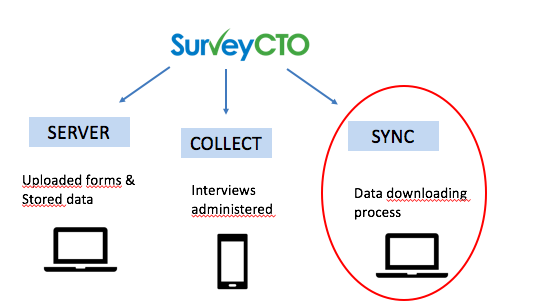
\includegraphics[width=\linewidth]{img/importscto}
	\end{figure}
\end{frame}


\begin{frame}[fragile]{1. Import SurveyCTO data to Stata}
\begin{multicols}{2}	
\begin{figure}
	\centering
	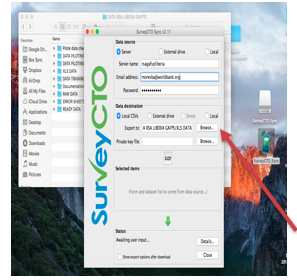
\includegraphics[width=\linewidth]{img/scto1}
\end{figure}
\begin{itemize}
	\item SurveyCTO Sync is the data download tool
	\item It is an application that sits on your local machine, and needs internet access to be able to download data	
	\item When you open it, this is what it looks like
	\item Step 1: Enter in the log-in details and the folder you would like to download the file to. Then click GO! 
\end{itemize}
\end{multicols}
\end{frame}



\begin{frame}[fragile]{1. Import SurveyCTO data to Stata}
\begin{multicols}{2}	
	\begin{figure}
		\centering
		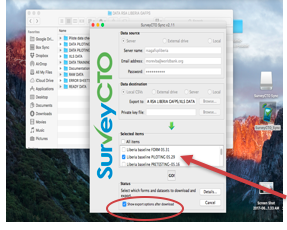
\includegraphics[width=\linewidth]{img/scto2}
	\end{figure}
	\begin{itemize}
		\item All of the forms that contain data will show up in the window at the bottom
		\item You may need to download all of them, or a single one
		\item In this example, I’m choosing to download just the pilot data. 
		\item Step 2: Select the form you want to download AND select the “Show export options after download” option at the bottom
			\begin{itemize}
				\item Note: you can always select this option later using the taskbar, but this will save you time
			\end{itemize}		 
	\end{itemize}
\end{multicols}
\end{frame}



\begin{frame}[fragile]{1. Import SurveyCTO data to Stata}
\begin{multicols}{2}	
	\begin{figure}
		\centering
		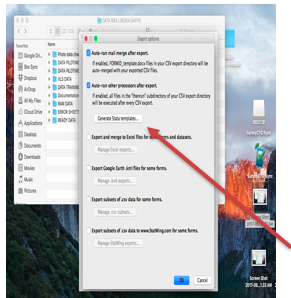
\includegraphics[width=\linewidth]{img/scto3}
	\end{figure}
	\begin{itemize}
		\item The ‘export options’ contain a number of different possibilities
		\item The one I wanted to show you about today is the STATA template that CTO generates to help set up your dataset
		\item Step 3: Click on the ‘Generate Stata templates…’ option	 
	\end{itemize}
\end{multicols}
\end{frame}



\begin{frame}[fragile]{1. Import SurveyCTO data to Stata}
\begin{multicols}{2}	
	\begin{figure}
		\centering
		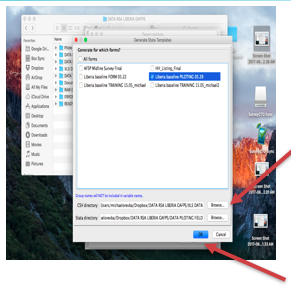
\includegraphics[width=\linewidth]{img/scto4}
	\end{figure}
	\begin{itemize}
		\item Once again, a number of different forms come up. Note that this includes forms not only from your current server, but your past work as well (this example has an AFSP project, as well as the Liberia Project)
		\item Another important aspect of this is what you choose as your CSV directory (the raw-est data) and your STATA directory
		\item This helps CTO write the do-file, so as to know where to open the raw data from, and where to save its DTA to
		\item Remember that we had already chosen the CSV directory earlier in the process, so this step is really about choosing the DTA location.
		\item Step 4: After you have selected the folder, click ‘OK’ 
	\end{itemize}
\end{multicols}
\end{frame}



\begin{frame}[fragile]{1. Import SurveyCTO data to Stata}
\begin{multicols}{2}	
	\begin{figure}
		\centering
		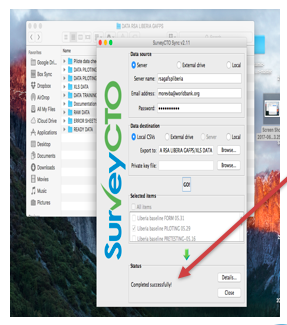
\includegraphics[width=\linewidth]{img/scto5}
	\end{figure}
	\begin{itemize}
		\item If everything has gone according to plan, you will see a ‘Completed successfully!’ message  
	\end{itemize}
\end{multicols}
\end{frame}


\begin{frame}[fragile]{1. Import SurveyCTO data to Stata}
\begin{multicols}{2}	
	\begin{figure}
		\centering
		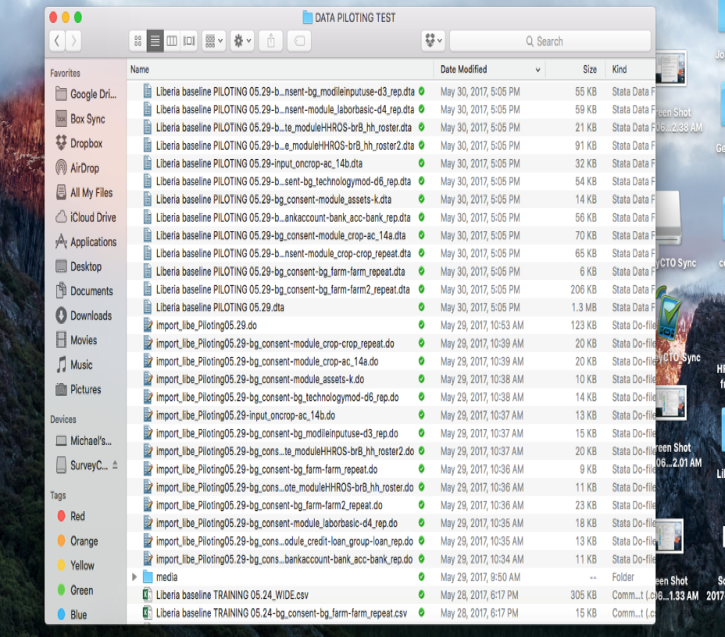
\includegraphics[width=\linewidth]{img/stata_dta}
	\end{figure}
	\begin{itemize}
		\item CTO will now export do-files into whatever folder you have asked it to export the dta-files into
		Remember that in this case CSVs are also being exported into that same folder
		\item Each repeat group has it’s own do-file, but there is also one do-file for the ‘master’ dataset i.e. all of the questions throughout your form that are not within any of the repeat groups
		Nested repeat groups will each have their own do-files too
		\item Step 5: Open your do-files and run them!		 
	\end{itemize}
\end{multicols}
\end{frame}


\begin{frame}[fragile]{1. Import SurveyCTO data to Stata}
\begin{multicols}{2}	
	\begin{figure}
		\centering
		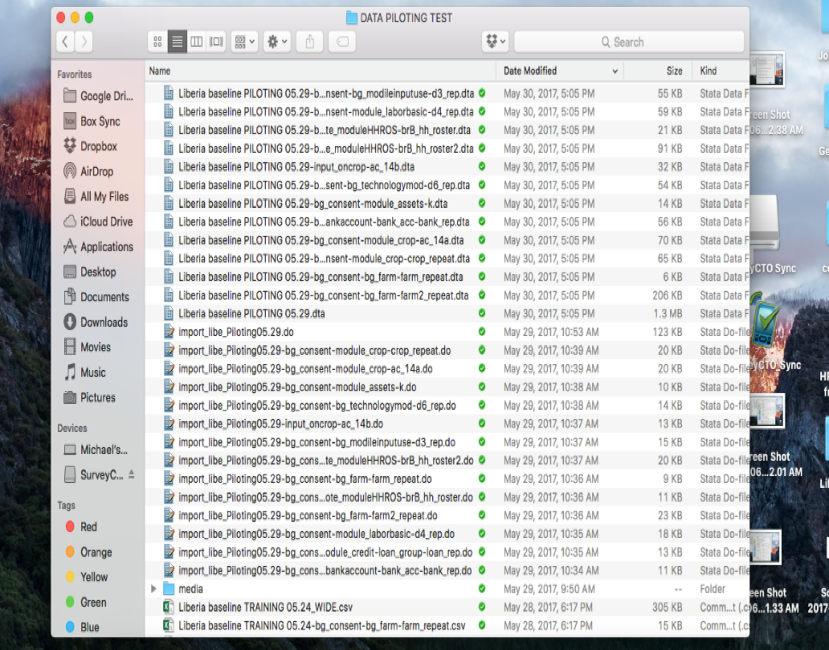
\includegraphics[width=\linewidth]{img/stata_dta2}
	\end{figure}
	\begin{itemize}
		\item .dta-files will now (not so) magically appear in that same destination folder!
		\item Voila!	 
	\end{itemize}
\end{multicols}
\end{frame}


\begin{frame}{Import Data to Stata}
\begin{itemize}
	\item Use Survey CTO’s file
		\begin{itemize}
			\item Takes labels from your questionnaire and add to your Stata data
		\end{itemize}
	\item Use code to filter only daily submissions
		\end{itemize}
\end{frame}


\begin{frame}{2. Duplicates}
\begin{itemize}
	\item Purpose: NONE! They’re there to make your life miserable
	\item Best to solve in real time!
		\begin{itemize}
			\item Much easer to solve the day after interview
				\begin{itemize}
					\item Enumerator still remembers the interview
					\item Field team still close to the respondent and can go back 
				\end{itemize}
		\end{itemize}
	\item We want to make sure all interviews are uploaded to the server. The only way to know how many interviews we have on the server is to first look for duplicates
	\item Other quality checks (back checks, high frequency checks, etc.) depend on uniquely identifying ID variables or are biased by duplicates
\end{itemize}
\end{frame}


\begin{frame}{ieduplicates}
\begin{itemize}
	\item Developed especially for, but not limited to, data downloaded from SurveyCTO servers
	\item Outputs a report in Excel. The report is also used to correct the duplicates in Stata
	\item Field supervisors without knowledge of Stata can make the corrections in the Excel file. The duplicates will be corrected next time you run the code
	\item The command always return the data set with the ID variable uniquely and fully identifying all observations
\end{itemize}
\end{frame}

\begin{frame}{ieduplicates - output}
	\begin{figure}
		\centering
		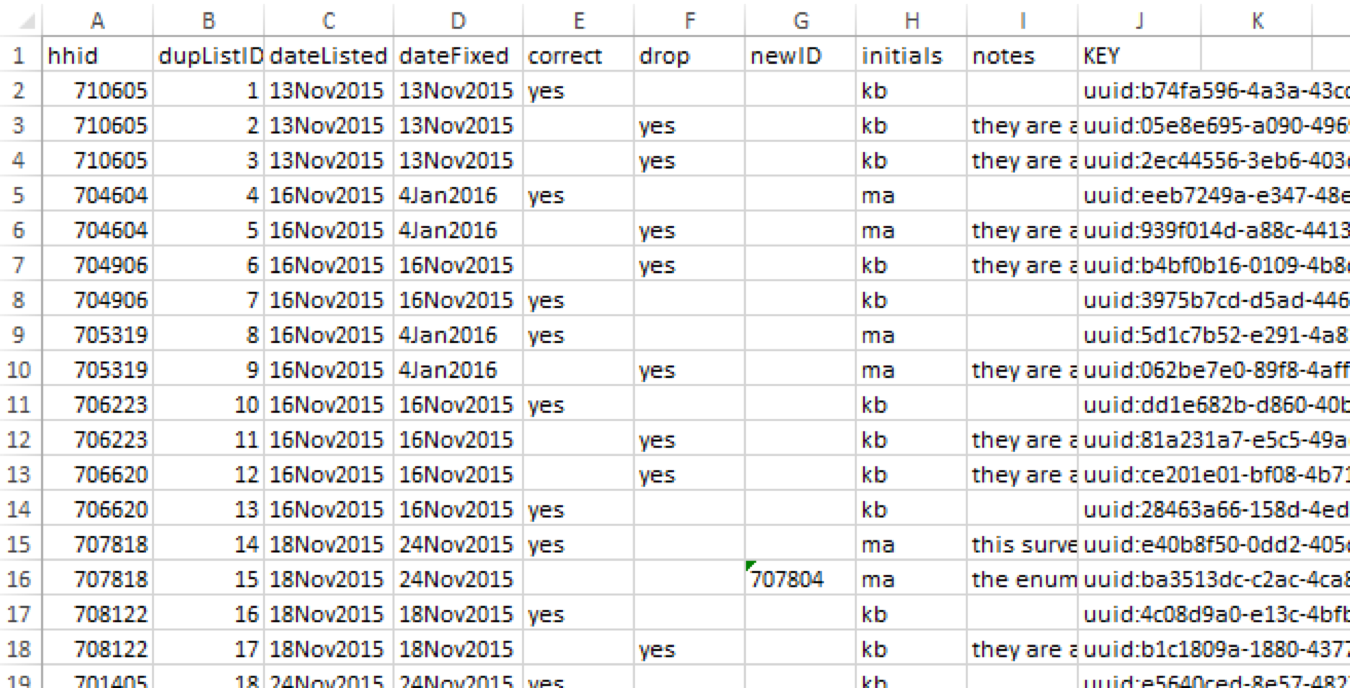
\includegraphics[width=\linewidth]{img/ieduplicates}
	\end{figure}
\end{frame}


\begin{frame}{Three main types of 
duplicates in SurveyCTO }
\begin{itemize}
	\item Type 1 - Double submissions of same observation and the same data
		\begin{itemize}
			\item First upload from tablet not complete due to bad internet
			\item Enumerator resends the form because he/she didn’t see the « successfuly sent » message
		\end{itemize}
	\item Type 2 - Double submissions of same observation but with modified data (rare in SurveyCTO)
		\begin{itemize}
			\item Answers modified after submission, and resubmitted
			\item Bad practice, more transparent to correct in a do-file
		\end{itemize}
	\item Type 3 - Incorrectly assigned ID. Two respondents are given the same ID
		\begin{itemize}
			\item Typo in field when entering respondent ID
		\end{itemize}
\end{itemize}
\end{frame}

\begin{frame}{Three main reasons for 
duplicates in SurvyeCTO }
\begin{itemize}
	\item Type 1 - Double submissions of same observation in the same data
	\begin{itemize}
		\item Few variables differs between the duplicates and differences are in submission date
	\end{itemize}
	\item Type 2 - Double submissions of same observation but modified data
	\begin{itemize}
		\item Some variables differs between the duplicates and some of them are in observation data
	\end{itemize}
	\item Type 3 - Incorrectly assigned ID. Two respondents are given the same ID
	\begin{itemize}
		\item Many variables differs between the duplicates and many of the differences are in observation data
	\end{itemize}
\end{itemize}
\end{frame}

\begin{frame}{iecompdup}
\begin{itemize}
	\item Compares all variables across a pair of duplicates and provide you with a list of the variables where the duplicates has different values. 
	\item From this information we can decide which type of duplicate
	\begin{itemize}
		\item If it is type 1 we can solve it immediately. 
		\item If it is type 3 then we are halfway to the solution
		\item Type 2 is rare. Re-evaluate if it is possible type 1 or type 3. Otherwise investigate.
	\end{itemize}
\end{itemize}
\end{frame}

\begin{frame}{}
\begin{itemize}
	\item To add:
		\begin{itemize}
			\item Type 1 is usually solved by looking at the data
			\item What to do if type 2 and type 3?
				\begin{itemize}
					\item Always requires an investigation together with field team
					\item Share report to supervisors asking what is the form to keep 
					\item You will soon find out which variables are important to investigate the duplicates, add them as keepvars() in ieduplicates
				\end{itemize}
		\end{itemize}
\end{itemize}
\end{frame}

\begin{frame}{ieduplicates}
\begin{itemize}
	\item Exercise 1
	\begin{itemize}
		\item install ieduplicates
		\item learn how to use ieduplicates
		\item practice identifying and correcting duplicates
	\end{itemize}
\end{itemize}
\end{frame}

\begin{frame}{HFC}
\begin{itemize}
	\item Given that you are in track 1, you are usually not expected to know how to write this, so we will focus on how to interpret
	\item We will not cover everything as that is responsibility of person writing
	\begin{itemize}
		\item There are templates that help with this
			\begin{itemize}
				\item IPA
				\item DIME is working
			\end{itemize}
	\end{itemize}
\end{itemize}
\end{frame}


\begin{frame}{3. Survey Log}
\begin{itemize}
	\item Make sure to keep records in the field that is updated very day with how many interviews that were completed
	\item Make sure that the number of observations on the server matches these records.
	\item Purpose: 
		\begin{itemize}
			\item Provide your team a quick overview of progress on the field
			\item Detect enumerators who are slacking
			\item Check balance if this is important for the survey (e.g. by gender)
		\end{itemize}
	\end{itemize}
\end{frame}


\begin{frame}{3. Survey Log}
\begin{itemize}
	\item Exercise 2 – Practice checking survey progress. Assume you’ve verified that the server matches the field log, i.e. no submissions are missing. 
\end{itemize}
\end{frame}


\begin{frame}{4. Back checks}
\begin{itemize}
	\item Purpose
		\begin{itemize}
			\item To monitor the quality of field work: Do some enumerators need extra support from supervisors?
			\item To understand whether your questionnaire accurately captures the key outcomes of your study: Do respondents understand the questions the way we intended to?
		\end{itemize}
	\item Best practices:
		\begin{itemize}
			\item ~ 10\% of surveys, 20\% in the first 2 weeks of field work
			\item Every team and every surveyor must be back checked 
			\item The back check sample must include a proportional number of missing and replacement respondents. 
			\item Selection of households for back checks must be random
		\end{itemize}
\end{itemize}
\end{frame}

\begin{frame}{Selecting Back Check Questions}
\begin{itemize}
	\item Type 1 variables 
		\begin{itemize}
			\item Straightforward questions where we expect very little variation
			\item E.g. education level, marital status, occupation, has children
		\end{itemize}
	\item Type 2 variables
		\begin{itemize}
			\item Questions where we expect capable enumerators to get the true answer
		\end{itemize}
	\item Type 3 variables
		\begin{itemize}
			\item Questions that we expect to be difficult. 
			\item Want to understand if these questions were interpreted in the field as intended		
		\end{itemize}
	\item Identifying Respondent and Interview Information
		\begin{itemize}
			\item Check if we have the right person; if the interview took place \& when
		\end{itemize}
\end{itemize}
\end{frame}

\begin{frame}{bcstats}
\begin{itemize}
	\item ssc install bcstats, replace
	\item Purpose:
	\begin{itemize}
		\item compares back check data and survey data, producing a data set of comparisons
		\item completes enumerator checks and stability checks for variables
	\end{itemize}
\end{itemize}
\end{frame}

\begin{frame}{Using bcstats report to improve data quality}
\begin{itemize}
	\item Type 1
		\begin{itemize}
			\item If >10\% discrepancies  - give surveyor a warning
			\item 20-30\% discrepancies - 2nd backcheck to determine who made errors
			\item If error is by surveyor  - audit 3 additional surveys by that surveyor in same week 
			\item if 20-30\% discrepancies -  put him/her on probation
			\item >40\% discrepancies - 2nd backcheck to determine who made errors and maybe re-survey HH 
			\item If surveyor made errors - re-survey HH \& audit all surveys done by surveyor in this batch
			\item If one more survey has 40\% discrepancies - fire surveyor immediately \& redo all his/her surveys with 20\% or more discrepancies
	\end{itemize}
\end{itemize}
\end{frame}

\begin{frame}{Using bcstats report to improve data quality}
\begin{itemize}
	\item Type 2
		\begin{itemize}
			\item >10\% discrepancies -> Consider re-training
			\item If one surveyor is responsible for more than 30\% of the errors in a single question, follow the steps for Type 1
		\end{itemize}
	\item Type 3
		\begin{itemize}
			\item Discuss >10\% with your survey team and your PIs. 
			\item PIs may decide to edit survey or add additional rounds
		\end{itemize}
\end{itemize}
\end{frame}

\begin{frame}{4. Backchecks}
\begin{itemize}
	\item Exercise 3
		\begin{itemize}
			\item Install bcstats
			\item Learn how to use bcstats
			\item Distinguish between types of backcheck variables 
			\item Explore bcstats output
		\end{itemize}
\end{itemize}
\end{frame}

%%%%%%%%%%%%%%%%%%%%%%%%%%%%%%%%%%%%%%%%%%% Final thougts section
\begin{frame}{Conclusion}


\vspace{20mm}
For more information or further questions please contact:
\newline John Doe (\url{johndoe@worldbank.org}) \newline Mary Doe (\url{marydoe@worldbank.org})

\end{frame}

%%%%%%%%%%%%%%%%%%%%%%%%%%%%%%%%%%%%%%%%%%% The End
\sectionpic{Thank You!}{img/section_slide}






\end{document} 